%------------------------------------
% Document Preamble
%------------------------------------
\documentclass[12pt, a4paper]{article}
\setlength{\oddsidemargin}{0.5cm}
\setlength{\evensidemargin}{0.5cm}
\setlength{\topmargin}{-1.6cm}
\setlength{\leftmargin}{0.5cm}
\setlength{\rightmargin}{0.5cm}
\setlength{\textheight}{24.00cm} 
\setlength{\textwidth}{15.00cm}
\parindent 0pt
\parskip 5pt
\pagestyle{plain}

%------------------------------------
% Imported packages
%------------------------------------
\usepackage{graphicx}
\usepackage{siunitx}

%------------------------------------
% Graphics path specification
%------------------------------------
\graphicspath{{./fig/}}

%------------------------------------
% Title block
%------------------------------------
\title{ENG720: Research Proposal}
\author{}
\date{}

\newcommand{\namelistlabel}[1]{\mbox{#1}\hfil}
\newenvironment{namelist}[1]{%1
\begin{list}{}
    {
        \let\makelabel\namelistlabel
        \settowidth{\labelwidth}{#1}
        \setlength{\leftmargin}{1.1\labelwidth}
    }
  }{%1
\end{list}}

\begin{document}
\maketitle

\begin{namelist}{xxxxxxxxxxxx}
\item[{\bf Title:}]
	To Be Confirmed
\item[{\bf Author:}]
	Shane Reynolds
\item[{\bf Supervisor:}]
	Charles Yeo
\item[{\bf Degree:}]
	Bachelor of Engineering (Honours)
\end{namelist}


%------------------------------------
% Contents
%------------------------------------
\tableofcontents
\newpage

%------------------------------------
% Introduction
%------------------------------------
\section{Introduction}
\subsection{Background}

\subsubsection{Power Systems and Frequency}
Interconnected power systems are comprised of power generating units and energy storage systems connected to transmission and distribution networks, where generated power is used to service load demand. A single line diagram of a power network can be seen in Figure 1. The left hand side of the diagram shows thermal generation units, such as coal and nuclear, in addition to renewable sources of generation, like wind and solar. The right hand side of the figure shows the distribution network and the consumers of generated energy: industry and households.
\begin{figure}[h]
	\centering
	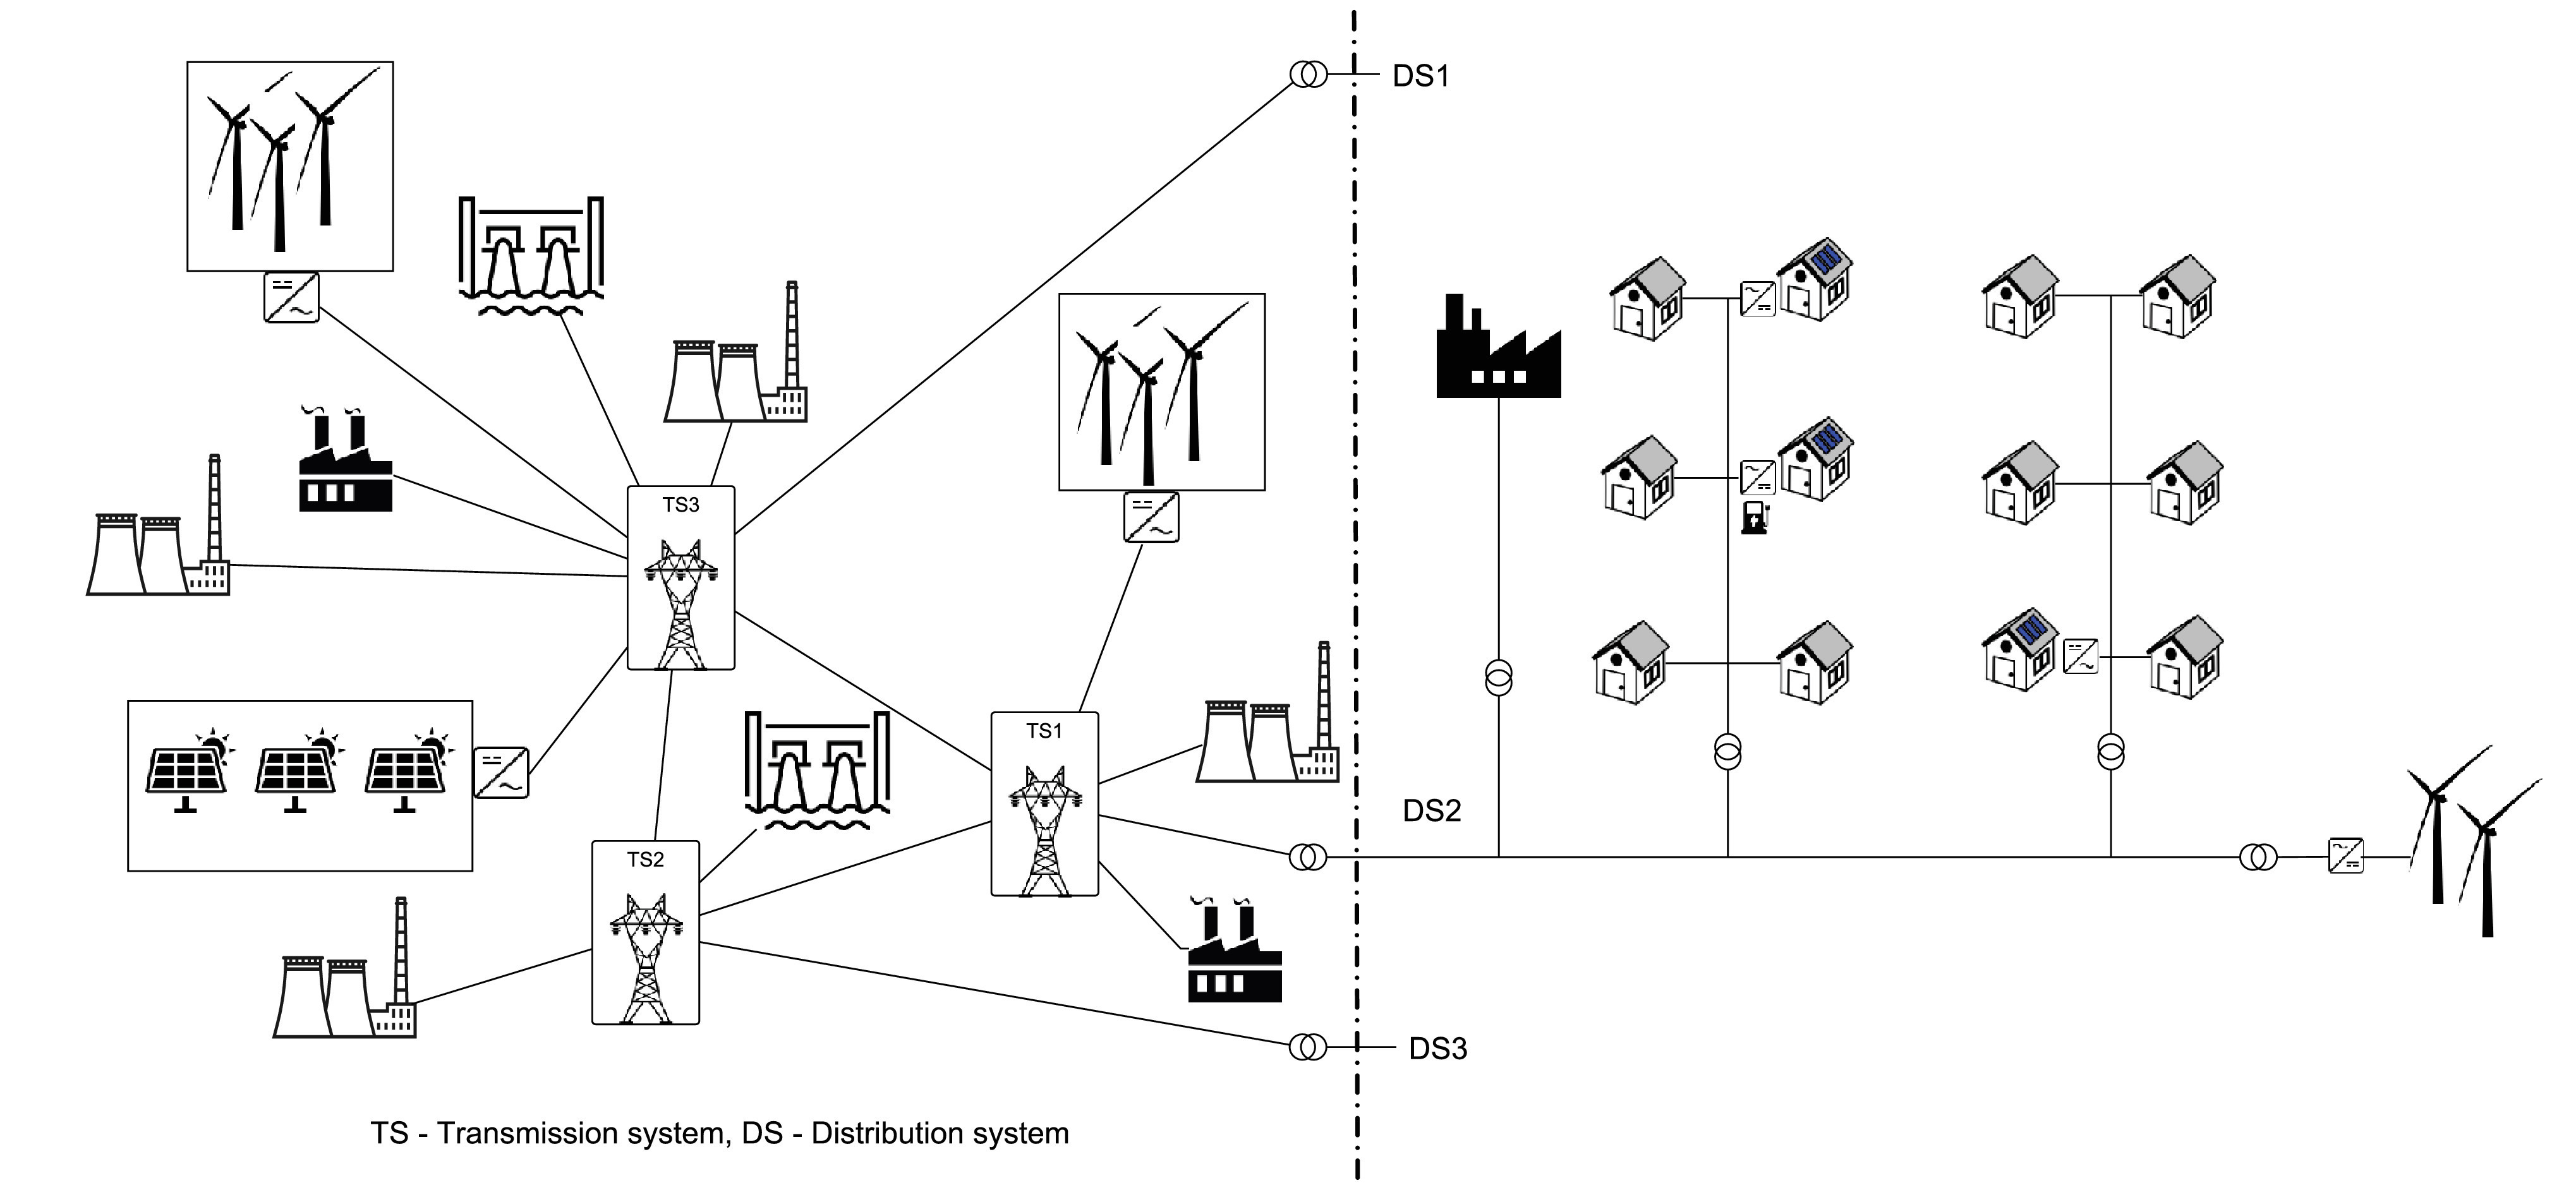
\includegraphics[scale=0.85]{power_system}
	\caption{A single line diagram of a typical power system taken from \cite{Glavic2019}. The image shows points of generation from thermal and renewable sources, and the subsequent supply of generated energy to meet load demand through the transmission and distribution network.}
\end{figure}

Successful operation of interconnected power systems requires total load demand to be matched with total generation, taking into account power losses involved with generation, transmission, and distribution \cite{Wood2013}. To understand why it is important to match generation with load demand it is useful to first consider the basic operation of a single thermal generator. A simple way to think about a thermal generator is consisting of a prime mover (turbine) and a synchronous machine, as depicted in Figure 2.
\begin{figure}[h]
\centering
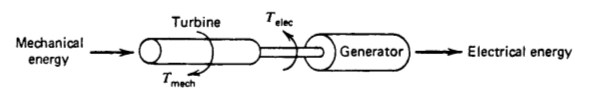
\includegraphics[height=1.4cm]{generation}
\caption{A thermal generation unit consists of a prime mover (turbine), and a synchronous machine. This image was taken from \cite{Wood2013}.}
\end{figure}

The prime mover provides mechanical torque, $T_{mech}$, which drives the synchronous machine producing electrical energy. In response, the synchronous machine creates a torque which opposes $T_{mech}$, dependent on the size of the load demand from households and industry. This is referred to as electrical torque and is denoted as $T_{elec}$. If $\alpha$ represents angular velocity of the generator rotating mass, and $I$ is the moment of inertia then by Newton's second law:
\begin{equation}
\sum T_i = I \alpha 
\end{equation}

Equation (1) shows that when $T_{mech}$ equals $T_{elec}$ the system will be in a steady state with zero angular acceleration, and a constant rotation at some angular velocity $\omega$. Now, if $T_{mech} > T_{elec}$, then the angular velocity $\omega$ of the system will increase as the system speeds up. Conversely, if $T_{mech} < T_{elec}$ then the angular velocity $\omega$ decrease as the system slows down. What makes this situation interesting is that at any point in time the total electrical load demand will fluctuate stochastically, meaning that an uncontrolled system will have a continually changing frequency. System controllers, such as the Australian Energy Market Operator (AEMO) and Power and Water Corporation (PWC), can forecast daily demand profiles with some reliability using historical data. An example of historical daily demand profiles are shown in Figure 3.  
\begin{figure}[h]
	\centering
	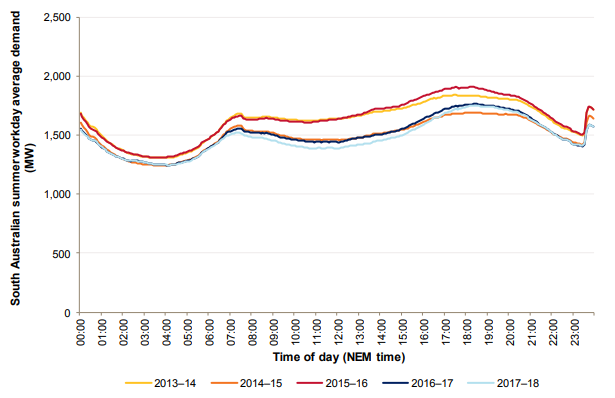
\includegraphics[height=7cm]{load_profile}
	\caption{Weekday energy demand profile in South Australia during summer \cite{AEMO2018}.}
\end{figure}

Forecasts provide a starting point that AEMO and PWC can use for estimating generation needed to meet demand for a given time. Unfortunately forecasts are not perfect and mismatches in generation and demand lead to small imbalances between $T_{mech}$ and $T_{elec}$, and thus a resulting in a change to angular velocity $\omega$ and the network frequency \cite{Glover2012}.\\ and unpredicted load appearing on the system appear on the system, or worse, generation assets could be disconnected from the network. 

Australia's electricity network is designed to operate at a frequency of 50$\si{\hertz}$. In the majority of network scenarios AEMO's desired operating range for frequency is between 49.85$\si{\hertz}$ and 50.15$\si{\hertz}$ \cite{AEMO2012}. The PWC Network Technical Code for the Northern Territory states that under normal operating conditions frequency should be maintained in the range 49.80$\si{\hertz}$ to 50.20$\si{\hertz}$ \cite{PWC2018}. Operation outside of specified ranges can cause damage to electrical equipment. Sustained over or under frequency will generally cause protection systems to remove equipment from the network, as will sudden large frequency deviations. If the disconnections are uncontrolled then this can create further imbalance to the electrical network. In order to correct these deviations, system controllers use generators which are referred to as regulating units. A regulating generator is a generator that has the capacity to increase or decrease mechanical torque $T_{mech}$ allowing the system controller to arrest changing frequency and restore the system to stable operating conditions. AEMO and PWC only require a subset of the generators on the network to act as regulating generators. TALK ABOUT SPINNING RESERVES. An example of regulation arresting a frequency disturbance, and the subsequent restoration of the system can be seen in Figure 4.
\begin{figure}[h]
\centering
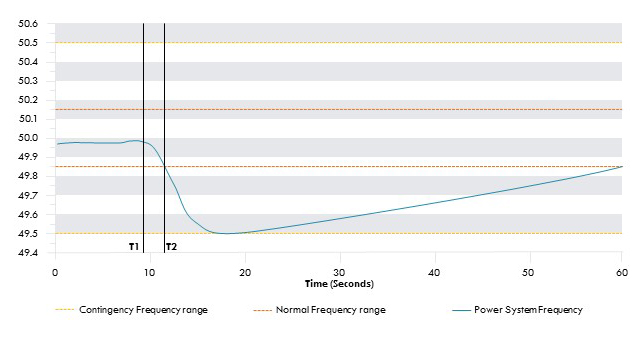
\includegraphics[height=8cm]{frequency_arrest}
\caption{text}
\end{figure}

Regulation needs to be performed quickly in response to a frequency disturbance. HOW QUICKLY DO UTILITIES NEED TO RESPOND. Typically regulation is performed automatically, except under highly abnormal operating conditions.

\subsubsection{Load frequency control for a single area}
The power system model shown in Figure 1 depicts total generation coming from many generation assets. Researchers often find it useful to divide generation assets into sub-groups referred to as control areas. Kothari defines a control area as a subset of generators belonging to a close knit area which constitute a coherent group such that all the generators speed up and slow down together maintaining their relative power angles \cite{Kothari2011}. The total network is therefore comprised of many interconnected control areas. An example of a series of interconnected control areas can be seen in Figure XXXX.
\begin{figure}[h]
	\centering
	
\includegraphics[scale=0.6]{placeholder}
	\caption{A number of control areas interconnected. Each control area is consists of many generators and loads.}
\end{figure}

To simplify analysis of interconnected systems, researchers tend to make a further simplifying assumption by representing all of the distinct generators in a control area as a single generator. This assumption also is made for loads in the control area. Figure XXXX depicts this assumption being applied to a control area with multiple generators and loads.
\begin{figure}[h]
\centering

\includegraphics[scale=0.6]{placeholder}
\caption{The left hand image shows a control area comprised of generators and loads. The right hand image shows the simplified control area which consists of a single generator and a single load.}
\end{figure}

The simplest power system to control frequency 
NEED TO TALK ABOUT CONSIDERING A SINGLE CONTROL AREA THAT HAS NO CONNECTION TO THE REST OF THE NETWORK

To control frequency of a single The regulation workhorse for a single control area, which performs the bulk of regulation activity, is the speed governor. These devices are connected to every generator and their operation in provision of frequency regulation is well understood.

\subsubsection{Two-area load frequency control}

DEFINE WHAT A TWO AREA CONTROL LOOKS LIKE

\begin{figure}[h]
	\centering
	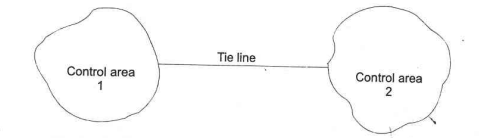
\includegraphics[scale=0.7]{two_area_system}
	\caption{Two area power system is comprised of generators and load connected via a tie line. Power flows from one area to the other depending on economic contracts.}
\end{figure}

TALK ABOUT WHAT HAPPENS IF WE JUST LET THE SPEED GOVENORS DO THE JOB

TALK ABOUT HOW THIS MAY END UP VIOLATING ECONOMIC CONTRACTS THAT ARE IN PLACE

INTRODUCE AUTOMATIC GENERATION CONTROL AND THE ITS PRIMARY MOTIVATION

TALK ABOUT THIS LARGELY BEING A SOLVED PROBLEM

\subsubsection{Reinforcement learning}

TALK ABOUT THE HISTORY OF REINFORCEMENT LEARNING

TALK ABOUT THE BASIC COMPONENTS OF HOW IT IS PUT TOGETHER

TALK ABOUT APPLICATIONS IN THIS FIELD

\subsubsection{Deep reinforcement learning}

TALK ABOUT HOW DRL DIFFERS TO STANDARD RL

TALK ABOUT THE BENEFITS OF USING THIS TYPE OF APPROACH


\subsection{Significance}

TALK ABOUT THE INCREASE OF RENEWABLES ENTERING THE SYSTEM

TALK ABOUT THE INCREASE OF HVDC TRANSMISSION TO NETWORK

TALK ABOUT THE INTRODUCTION OF EV IN THE COMING DECADES AND THE IMPLCATIONS FOR THE ELECTRICAL NETWORK

TALK ABOUT A DECENTRALISED GENERATION MODEL THROUGH THE USE OF VIRTUAL POWER NETWORKS WHICH ARE COMPRISED OF MULTIPLE ROOFTOP SOLAR ASSETS

TALK ABOUT THE DRAWBACKS TO ASSUMING LINEAR MODELS WITH TRADITIONAL CONTROL METHODS - THIS IS PROBLEMATIC SINCE ANY SIMULATION OF THE SYSTEM WOULD BE USING LINEAR MODELS TO SIMULATE THE SYSTEM DYNAMICS - DRL CONTROL WOULD BE BASED ON A LINEARISED SYSTEM

Why is this topic significant to you? Why should others be interested in it? You might find it helpful to think about what led you to undertake research in this area. You might also consider how scholars in the field discuss its importance. In what ways is your understanding of its significance similar or different?


%------------------------------------
% Research Aims and Questions
%------------------------------------
\section{Research Aims and Questions}
Now state explicitly the hypothesis you aim to test. Make references to the items listed in the Reference section that back up your arguments for why this is a reasonable hypothesis to test, for example the work of Knuth.

Explain what you expect will be accomplished by undertaking this particular project.  Moreover, is it likely to have any other applications?

Constructing a clear and focused research question (or questions) is crucial to producing a good research proposal and, more importantly, shaping the direction of your research. The question indicates exactly what you want to explore and allows the reader to assess whether or not your project is viable. It also gives the reader a sense of the arguments or findings that you might produce in response. This allows them to provide you with useful feedback on the direction of your research.

The criteria for a good research question vary from one field of study to another. It is therefore advisable that you consult with your supervisor and closely examine examples from other theses and published studies to get a sense of the requirements in your field. In general terms, however, a good research question should be:
\begin{itemize}
\item Relevant: It must clearly relate to the problems or issues that the project seeks to address.
\item Important: It should address a key problem in the field (see From identifying a gap to constructing a problem above).  
\item Clear: It should be expressed using concise language and contain no ambiguity.
\item Precise: What is being investigated should be clearly specified.
\item Researchable: The information and sources required to answer the question must exist and you must be able to access them (with the exception of data that you will generate yourself through surveys, experiments, etc.).
\end{itemize}

In cases where there is more than one research question, the questions must be clearly related to each other so that they add up to a coherent whole.

\subsection{Constructing a Research Question}
The wording of your research question (or questions) is important because it will direct your approach and writing and help to shape the feedback that you receive from readers of your proposal. It is important to understand that you can change your research question at a later date if you think that the wording needs to be changed or if you make discoveries that encourage a different approach to the topic. It is highly likely, in fact, that the question that you pose in your proposal will be different from the question or questions that your thesis actually answers.

Wording of research questions can vary significantly from one field of study to another, so it is advisable that you consult with your supervisor and seek out examples from other research proposals, theses, or published papers. However, the following general points can be made:

\begin{itemize}
\item How and why questions are usually preferred as they generate analytical rather than descriptive findings.
\item The question should be worded in such a way that a number of different responses would be possible.
\item The wording should be neutral in tone. Avoid value judgements or untested assumptions.
\item The wording should include the key concepts and relationships that you have identified.
\end{itemize}

\subsection{Interrogate Research Question}
After the initial drafting of your research question you should interrogate it to highlight strengths and weaknesses in your thinking or wording. Write responses to the following questions: 

\begin{itemize}
\item Does this research question interest me? Will it sustain my interest?
\item Does this question help to address a significant research problem?
\item Has this question already been answered by others? If so, how will my response differ?
\item Is the question too easy to answer? Is the answer too obvious? 
\item Can the question be approached from different angles? 
\item Will this question allow me to generate a strong and interesting position or findings? At this point in time what hypothesis would I make in response to the question?
\item Does the question have an appropriate scope? Is the specified content too broad or too narrow? 
Is the question researchable? 
\item What kind of information and sources will I need to answer the question?  Am I able to access this information? Will I need to generate my own data?  
\item What about the ethics of the question? Does it entail risks for the researcher or (if relevant) the participants? 
\end{itemize}


%------------------------------------
% Literature Review
%------------------------------------
\section{Literature Review}
The literature review surveys key academic works in your field of research, such as books, refereed journal articles, and postgraduate theses. The review should summarise, analyse, categorise and compare the most significant works - it does not need to cover everything that has been written on the topic. Most importantly, it should clearly demonstrate the gap or problem that your research project will address by outlining both the strengths and the limitations of previous research.

\subsection{Planning and Writing a Literature Review}

There are three main considerations when writing a literature review for a research proposal:

\begin{itemize}
\item Focus: A literature review for a research project should give an accurate picture of the general field, but rather than discuss every text in detail it should focus on works that are directly related to your specific topic. It is usually best to focus on the most prominent and recent contributions to the topic.
\item Structure: Rather than discuss each selected text separately, a literature review should be organised around key similarities, differences, and other points that you want to make about the development of academic writing on the topic. Search for a review article on the topic (a kind of literature review found in refereed journals) and study the literature reviews contained in recently published books and journal articles on the topic. Consider how these authors categorise and evaluate the literature.
\item Faculty/School specifics: The above points apply for most research proposals, but some faculties and schools will have their own requirements regarding the content and word count of the literature review component. This will have an influence on how you select and critique the literature. It is therefore important that you check the specific requirements of your Faculty or School.
\end{itemize}

\subsection{Brainstorming for a Literature Review}
A useful way to generate ideas for your literature review is to brainstorm the key scholars, texts, arguments, sources and methods that are related to your research topic. Write down responses to the following questions. Your answers might take the form of brief dot points or you might prefer to write more extensive responses. Extensive responses are often a useful way of thinking through a question or issue that you find challenging:
\begin{itemize}
\item Have scholars attempted to address the research gap or problem that I intend to explore?
	\begin{itemize}
		\item If so, how have they attempted to address it? Can I place them into different categories?
		\item If not, why not?
	\end{itemize}
\item How and why are the approaches of key scholars similar? How and why are their approaches different?
\end{itemize}

Consider similarities and differences in:
\begin{itemize}
\item Theoretical frameworks
\item The sources and data used
\item Research methods (e.g. quantitative, qualitative, experimental, mixed-method)
\item What are the strengths of research on this topic?
\item What are the limitations, gaps and weaknesses in the field?
\end{itemize}


%------------------------------------
% Project Design
%------------------------------------
\section{Project Design}
In this section of your proposal you will need to answer three questions:
\begin{itemize}
\item What kind of data or sources will you use?
\item How will you collect and manage this material?
\item Which theoretical and methodological techniques will you use to interpret and analyse these data/sources?
\end{itemize}

It is important that you explain the design of your project in a clear and logical way. Your reader should be able to clearly see what you will do and how will you do it, and how this combination of data/sources and methods will allow you to address your research problem.

\subsection{Tips for completing the study/project design component}
The most important thing to keep in mind about the study/project design component is that it should not simply consist of a list of tasks that will be undertaken. Above all, it needs to establish that these tasks constitute the most effective way of exploring the research problem.

The key to composing a clear and focused study/project design is to show how you are building upon and/or departing from the theoretical and methodological approaches of key scholars in the field. It is therefore necessary to:
\begin{itemize}
\item Consider the theories and methods that other researchers have used, and;
\item Consider the theories and methods that have not been used (or that have been underutilised) but perhaps could be.
\end{itemize}

When writing up your study/project design, be specific about:
\begin{itemize}
\item The methods that you will use to gather your information;
\item The theories and techniques you will use to analyse the information
\item The relevance of these approaches to your research problem
\end{itemize}

Specify the particular activities that you will undertake and show how they will contribute to the investigation of your research problem (e.g. “I will engage in a close content analysis of political satire in order to show how it subverts the visual and rhetorical tropes of ‘serious’ political discourse”).

Finally, anticipate any potential barriers that you will face in carrying out your research design. No method is perfect, so you need to describe what the shortcomings will be and explain how you will address them.

\subsection{Brainstorm your study design}

The following questions will help you to formulate your study/project design. You might find it useful to organise your responses into a table, mind-map, or flow-chart (see example below). Many researchers prefer this approach as it allows them to visualise their project in its entirety, and draw connections between data and research goals that they may not have previously considered.
\begin{itemize}
\item What is your research problem?
\item What are the specific research goals or questions that you will need to address in order to investigate this problem?
\item What kind of data or sources will best allow you to reach these goals?
\item How will you gather your data/sources/information? How will you gain access to them? Will you need to generate your own data by conducting surveys or experiments?
\item What method or methods of interpretation and analysis is most suitable for your project? Will your study be qualitative, quantitative, or mixed-method?
\item What theories underlie your research? How will these theories allow you to meet your research goals?
\item Are there any ethical implications of your data collection or method of analysis?
\end{itemize}


%------------------------------------
% Timeline
%------------------------------------
\section{Timeline}
The timeline demonstrates to the reader that your project can be completed within the period of candidature. The timeline should consist of a series of goals that you will need to meet in order to complete all aspects of your thesis, from initial research to the final editing, with an expected date of completion for each step. It should also contain a statement of the progress that you have made to date. The timeline should also factor in other research related activities such as conferences and publications (if applicable).

The timeline is not a static document; you will need to update it regularly.


%------------------------------------
% Expected Outcomes and Impacts
%------------------------------------
\section{Expected Outcomes and Impacts}
Conclude your research proposal by stating your expected outcomes. At this stage in the research process, what arguments and conclusions do you expect to reach? Your reader will understand that these are projected outcomes based on the extent of research at the time of writing, and that they will almost certainly change in the light of further research. It is essential, however, that you give your reader a sense of what conclusions may be drawn. This will allow your reader to further assess the significance and validity of your project. It will also indicate to your reader that you have thought ahead and considered the potential outcomes and implications of your research.

To avoid repetition with the description of your research aims and significance earlier in the proposal, focus on how you envisage your research will contribute to debates and trends in your field. What impact might your findings have on how the problem is perceived? What impact might your methods have on how research is conducted in the future?


%------------------------------------
%Bibliography
%------------------------------------
\bibliographystyle{unsrt}
\bibliography{./bib/my_bib}

\end{document}